\chapter{Introducci\'on y conceptos previos}
\section{Introducci\'on}
Hasta finales de 1988 muy poca gente tomaba en serio el tema de la seguridad en
redes de computadores de prop\'osito general. Mientras que por una parte 
Internet iba 
creciendo exponencialmente con redes importantes que se adher\'{\i}an a ella, 
como {\sc bitnet} o {\sc hepnet}, por otra el auge de la inform\'atica de 
consumo (hasta la d\'ecada de los ochenta muy poca gente se pod\'{\i}a permitir
un ordenador y un m\'odem en casa) unido a factores menos t\'ecnicos (como la
pel\'{\i}cula {\it Juegos de Guerra}, de 1983) iba produciendo un aumento 
espectacular en el n\'umero de piratas inform\'aticos.\\
\\Sin embargo, el 22 de noviembre de 1988 Robert T. Morris protagoniz\'o el
primer gran incidente de la seguridad inform\'atica: uno de sus programas se
convirti\'o en el famoso {\it worm} o gusano de Internet. Miles de ordenadores
conectados a la red se vieron inutilizados durante d\'{\i}as, y las p\'erdidas 
se estiman en millones de d\'olares. Desde ese momento el tema de la seguridad 
en sistemas operativos y redes ha sido un factor a tener muy en cuenta por 
cualquier responsable o administrador de sistemas inform\'aticos.
Poco despu\'es de este incidente, y a la vista de los potenciales peligros que
pod\'{\i}a entra\~nar un fallo o un ataque a los sistemas inform\'aticos 
estadounidenses (en general, a los sistemas de cualquier pa\'{\i}s) la agencia
{\sc darpa} ({\it Defense Advanced Research Projects Agency}) cre\'o el {\sc 
cert} ({\it Computer Emergency Response Team}), un grupo formado en su mayor
parte por voluntarios cualificados de la comunidad inform\'atica, cuyo objetivo
principal es facilitar una respuesta r\'apida a los problemas de seguridad que
afecten a {\it hosts} de Internet (\cite{kn:den90}).\\
\\Han pasado m\'as de diez a\~nos desde la creaci\'on del primer {\sc cert}, y
cada d\'{\i}a se hace patente la preocupaci\'on por los temas relativos a la
seguridad en la red y sus equipos, y tambi\'en se hace patente la necesidad de
esta seguridad. Los piratas de anta\~no casi han desaparecido, dando paso a
nuevas generaciones de intrusos que forman grupos como {\it Chaos Computer Club}
o {\it Legion of Doom}, organizan encuentros como el espa\~nol Iberhack, y 
editan revistas o {\it zines} electr\'onicos ({\it 2600: The Hacker's Quartely}
o {\it Phrack} son quiz\'as las m\'as conocidas, pero no las \'unicas). Todo 
esto con un objetivo principal: compartir conocimientos. Si hace unos a\~nos 
cualquiera que quisiera adentrarse en el mundo {\it underground} casi no 
ten\'{\i}a m\'as remedio que conectar a alguna BBS donde se tratara el tema, 
generalmente
con una cantidad de informaci\'on muy limitada, hoy en d\'{\i}a tiene a su 
disposici\'on gigabytes de informaci\'on electr\'onica publicada en Internet; 
cualquier aprendiz de pirata puede conectarse a un servidor {\it web}, descargar
un par de programas y ejecutarlos contra un servidor desprotegido... con un 
poco de (mala) suerte, esa misma persona puede conseguir un control total sobre
un servidor Unix de varios millones de pesetas, probablemente desde su PC con
Windows 98 y sin saber nada sobre Unix. De la misma forma que en su d\'{\i}a 
{\it Juegos de Guerra} cre\'o una nueva generaci\'on de piratas, en la segunda 
mitad de los noventa pel\'{\i}culas como {\it The Net}, {\it Hackers} o {\it Los
Corsarios del Chip} han creado otra generaci\'on, en general mucho menos 
peligrosa que la anterior, pero cuanto menos, preocupante: aunque sin grandes
conocimientos t\'ecnicos, tienen a su disposici\'on multitud de programas y 
documentos sobre seguridad (algo que los piratas de los ochenta apenas 
pod\'{\i}an imaginar), adem\'as de ordenadores potentes y conexiones a Internet
baratas. Por si esto fuera poco, se ven envalentonados a trav\'es de sistemas
de conversaci\'on como el IRC ({\it Internet Relay Chat}), donde en canales como
{\tt \#hack} o {\tt \#hackers} presumen de sus logros ante sus colegas. 
\section{Justificaci\'on y objetivos}
A la vista de lo comentado en el primer punto, parece claro que la seguridad de
los equipos Unix ha de ser algo a considerar en cualquier red. Diariamente 
por cualquiera de ellas circulan todo tipo de datos, entre ellos muchos que se 
podr\'{\i}an catalogar como {\it confidenciales} (n\'ominas, expedientes, 
presupuestos\ldots) o al menos
como {\it privados} (correo electr\'onico, proyectos de investigaci\'on, 
art\'{\i}culos a punto de ser publicados\ldots). Independientemente de la 
etiqueta que cada
usuario de la red quiera colgarle a sus datos, parece claro que un fallo de
seguridad de un equipo Unix o de la propia red no beneficia a nadie, y mucho 
menos a la imagen de nuestra organizaci\'on. Y ya no se
trata simplemente de una cuesti\'on de imagen: seg\'un el {\it  Computer 
Security Institute}, en su encuesta de 1998, las p\'erdidas econ\'omicas 
ocasionadas por delitos relacionados con nuevas tecnolog\'{\i}as 
(principalmente accesos internos no autorizados) s\'olo en 
Estados Unidos ascienden anualmente a m\'as 20.000 millones de pesetas, cifra
que cada a\~no se incrementa en m\'as del 35\%; los delitos inform\'aticos
en general aumentan tambi\'en de forma espectacular a\~no tras a\~no, alcanzando
incluso cotas del 800\% (\cite{kn:san82}).\\
\\A lo largo de este trabajo se va a intentar hacer un repaso de los puntos 
habituales referentes a seguridad en Unix y redes de computadores (problemas, 
ataques, defensas\ldots), aplicando el estudio a entornos con requisitos de 
seguridad medios (universidades, empresas, proveedores de acceso a 
Internet\ldots); de esta forma se ofrecer\'a una perspectiva general de la 
seguridad en
entornos Unix, el funcionamiento de sus mecanismos, y su correcta utilizaci\'on.
Tambi\'en se hablar\'a, en menor medida, sobre temas menos t\'ecnicos
pero que tambi\'en afectan directamente a la seguridad inform\'atica, como 
puedan ser el problema del personal o la legislaci\'on vigente.\\
\\El objetivo final de este proyecto ser\'{\i}a marcar unas pautas para 
conseguir un nivel de seguridad {\bf aceptable} en los sistemas Unix conectados
en cualquier red,
entendiendo por `aceptable' un nivel de protecci\'on suficiente para que la 
mayor\'{\i}a de potenciales intrusos interesados en los equipos de nuestra
organizaci\'on fracasara ante un ataque contra los mismos. Obviamente, es 
imposible garantizar una plena seguridad ante cualquier atacante: seguramente
un pirata experimentado, con el tiempo suficiente, pagado, o simplemente muy 
interesado en uno de nuestros equipos, no tendr\'{\i}a muchos problemas en 
acceder a \'el. Este hecho, aunque preocupante, es casi inevitable; lo evitable
es que cualquier persona sea capaz de atacar con \'exito un equipo simplemente 
por haber visto una pel\'{\i}cula, descargado un par de p\'aginas {\it web} y 
ejecutado un programa que ni ha hecho ni entiende.\\
\\Por supuesto, este proyecto no pretende ser en ning\'un momento una ayuda 
para la gente que est\'e interesada en atacar m\'aquinas Unix o subredes 
completas, ni tampoco una invitaci\'on a hacerlo. 
Aunque por su naturaleza la informaci\'on aqu\'{\i} presentada 
puede ser utilizada para da\~nar sistemas inform\'aticos (como cualquier 
informaci\'on sobre seguridad inform\'atica), no es ese su 
prop\'osito sino, como hemos dicho, incrementar la seguridad de los sistemas
Unix y las redes en las que \'estos se ubican. Por tanto va a intentar estar 
escrito de forma que no
se pueda utilizar f\'acilmente como una {\it `receta de cocina'} para {\it 
crackers}; si alguien quiere un documento sobre c\'omo atacar 
sistemas, puede dejar de leer este trabajo y buscar en Internet informaci\'on 
sobre ese tema. Conseguir romper la seguridad de un sistema de forma no 
autorizada 
es, en la mayor\'{\i}a de los casos, un s\'{\i}mbolo de inmadurez, y por 
supuesto ni denota inteligencia ni unos excesivos conocimientos: si alguien se
considera superior por acceder ilegalmente a una m\'aquina utilizando un
programa que ni ha hecho ni es capaz de entender, que revise
sus principios, y si tras ha\-cer\-lo a\'un piensa lo mismo, que dedique
su {\it inteligencia} y sus {\it conocimientos} a tareas que ayuden a 
incrementar la seguridad, como la construcci\'on de sistemas de autenticaci\'on 
fiables y baratos o el dise\~no de nuevos criptosistemas seguros. {\bf
Eso} es seguridad inform\'atica, y no lo que habitualmente se nos quiere hacer
creer: la seguridad inform\'atica no consiste en conocerse todos los {\it bugs}
de un sistema operativo, con sus correspondientes {\it exploits} ni en jugar 
a {\it superjakers} en canales de {\sc IRC}. Lamentablemente, este es
el panorama de la {\it seguridad} m\'as visible en Espa\~na en la actualidad;
esperemos que alg\'un d\'{\i}a cambie.
\section{>Qu\'e es {\it seguridad}?}
Podemos entender como {\bf seguridad} una caracter\'{\i}stica de cualquier 
sistema (inform\'atico o no) que nos indica que ese sistema est\'a libre de 
todo peligro, da\~no o riesgo, y que es, en cierta manera, infalible. Como 
esta caracter\'{\i}stica, particularizando para el caso de sistemas operativos
o redes de computadores, es muy dif\'{\i}cil de conseguir (seg\'un la 
mayor\'{\i}a de expertos, imposible), se suaviza la definici\'on de {\it 
seguridad} y se pasa a hablar de {\bf fiabilidad} (probabilidad de que un 
sistema se comporte tal y como se espera de \'el) m\'as 
que de {\it seguridad}; por tanto, se habla de {\it sistemas fiables} en lugar 
de hacerlo de {\it sistemas seguros}.\\
\\A grandes rasgos se entiende que mantener un sistema {\it seguro} (o 
fiable) consiste b\'asicamente en garantizar tres aspectos (\cite{kn:pfl97}):
confidencialidad, integridad y disponibilidad. Algunos estudios 
(\cite{kn:lap91},\cite{kn:olo92}\ldots) integran la seguridad dentro de una
propiedad m\'as general de los sistemas, la {\bf confiabilidad}, entendida como
el nivel de calidad del servicio ofrecido. Consideran la disponibilidad como 
un aspecto al mismo nivel que la seguridad y no como parte de ella, por lo que 
dividen esta \'ultima en s\'olo las dos facetas restantes, confidencialidad e 
integridad. En este trabajo no seguiremos esa corriente por considerarla 
minoritaria.\\
\\>Qu\'e implica cada uno de los tres aspectos de los que hablamos? La {\bf
confidencialidad} nos dice que los objetos de un sistema han de ser accedidos 
\'unicamente por elementos autorizados a ello, y que esos elementos autorizados
no van a convertir esa informaci\'on en disponible para otras entidades; la 
{\bf integridad} significa que los objetos s\'olo pueden ser 
modificados\footnote{Por {\it modificar} entendemos escribir, cambiar, cambiar
el estado, borrar y crear.} por elementos autorizados, y de una manera 
controlada, y la {\bf disponibilidad} indica que los objetos del sistema tienen 
que permanecer accesibles a elementos autorizados; es el contrario de la 
{\bf negaci\'on de servicio}. Ge\-ne\-ral\-men\-te tienen que existir los tres 
aspectos
descritos para que haya seguridad: un sistema Unix puede conseguir
confidencialidad para un determinado fichero haciendo que ning\'un usuario (ni
siquiera el {\it root}) pueda leerlo, pero este mecanismo no proporciona 
disponibilidad alguna.\\
\\Dependiendo del entorno en que un sistema Unix trabaje, a sus responsables
les interesar\'a dar prioridad a un cierto aspecto de la seguridad. Por ejemplo,
en un sistema militar se antepondr\'a la confidencialidad de los datos 
almacenados o
transmitidos sobre su disponibilidad: seguramente, es preferible que alguien
borre informaci\'on confidencial (que se podr\'{\i}a recuperar despu\'es desde
una cinta de {\it backup}) a que ese mismo atacante pueda leerla, o a que esa
informaci\'on est\'e disponible en un instante dado para los usuarios 
autorizados. En cambio, en un servidor NFS de un departamento se premiar\'a la
disponibilidad frente a la confidencialidad: importa poco que un atacante lea
una unidad, pero que esa misma unidad no sea le\'{\i}da por usuarios 
autorizados va a suponer una p\'erdida de tiempo y dinero. En un entorno 
bancario, la faceta que m\'as ha de preocupar a los responsables del sistema
es la integridad de los datos, frente a su disponibilidad o su confidencialidad:
es menos grave\footnote{Aunque por supuesto no es en absoluto recomendable.} 
que un usuario consiga leer el saldo de otro que el hecho de que ese usuario 
pueda modificarlo.
\section{>Qu\'e queremos proteger?}
Los tres elementos principales a proteger en cualquier sistema inform\'atico son
el {\it software}, el {\it hardware} y los datos. Por {\bf hardware} entendemos
el conjunto formado por todos los elementos f\'{\i}sicos de un sistema 
inform\'atico, como CPUs, terminales, cableado, medios de almacenamiento 
secundario (cintas, CD-ROMs, diskettes\ldots) o tarjetas de red. Por {\bf 
software} entendemos el conjunto de programas l\'ogicos que hacen funcional al 
{\it hardware}, tanto sistemas operativos como aplicaciones, y por {\bf datos}
el conjunto de informaci\'on l\'ogica que manejan el {\it software} y el {\it
hardware}, como por ejemplo paquetes que circulan por un cable de red o entradas
de una base de datos. Aunque generalmente en las auditor\'{\i}as de seguridad
se habla de un cuarto elemento a proteger, los {\bf fungibles} (elementos que
se gastan o desgastan con el uso cont\'{\i}nuo, como papel de impresora, {\it 
t\'oners}, cintas magn\'eticas, {\it diskettes}\ldots), aqu\'{\i} no 
consideraremos la seguridad de estos elementos por ser externos al sistema 
Unix.\\
\\Habitualmente los datos constituyen el principal elemento de los tres a 
proteger, ya que es el m\'as amenazado y seguramente el m\'as dif\'{\i}cil de 
recuperar\footnote{Quiz\'as no el m\'as caro, pero s\'{\i} el m\'as 
dif\'{\i}cil.}: 
con toda seguridad una m\'aquina Unix est\'a ubicada en un lugar de 
acceso f\'{\i}sico restringido, o al menos controlado, y adem\'as en caso de
p\'erdida de una aplicaci\'on (o un programa de sistema, o el propio n\'ucleo
de Unix) este {\it software} se puede restaurar sin problemas desde su medio
original (por ejemplo, el CD-ROM con el sistema operativo que se utiliz\'o para
su instalaci\'on). Sin embargo, en caso de p\'erdida de una base de datos o de
un proyecto de un usuario, no tenemos un medio `original' desde el que 
restaurar: hemos de pasar obligatoriamente por un sistema de copias de 
seguridad, y a menos que la pol\'{\i}tica de copias sea muy estricta, es 
dif\'{\i}cil devolver los datos al estado en que se encontraban antes de la 
p\'erdida.\\
\\Contra cualquiera de los tres elementos descritos anteriormente (pero 
principalmente sobre los datos) se pueden realizar multitud de ataques o, dicho
de otra forma, est\'an expuestos a diferentes amenazas. Generalmente, la 
taxonom\'{\i}a m\'as elemental de estas amenazas las divide en cuatro grandes
grupos: interrupci\'on, interceptaci\'on, modificaci\'on y fabricaci\'on. 
Un ataque se clasifica como {\bf interrupci\'on} si hace que un objeto del
sistema se pierda, quede inutilizable o no disponible. Se tratar\'a de una
{\bf interceptaci\'on} si un elemento no autorizado consigue un acceso a un 
determinado objeto del sistema, y de una {\bf modificaci\'on} si adem\'as de
conseguir el acceso consigue modificar el objeto; algunos autores 
(\cite{kn:olo92}) consideran un caso especial de la modificaci\'on: la {\bf
destrucci\'on}, entendi\'endola como una modificaci\'on que inutiliza al 
objeto afectado. Por \'ultimo, se dice que un ataque es una {\bf fabricaci\'on} 
si se trata de una modificaci\'on destinada a conseguir un objeto similar al 
atacado de forma que sea dif\'{\i}cil distinguir entre el objeto original y 
el `fabricado'. En la figura \ref{ataques} se muestran estos tipos de ataque
de una forma gr\'afica.
\begin{figure}
\vspace{0.7cm}
\begin{center}
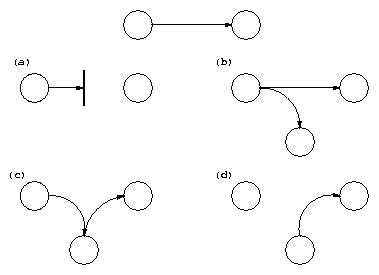
\includegraphics{attacks.png}
\end{center}
\caption{Flujo normal de informaci\'on entre emisor y receptor y posibles
amenazas: (a) inter\-rupci\'on, (b) interceptaci\'on, (c) modificaci\'on y (d) 
fabricaci\'on.}
\label{ataques}
\end{figure}
\section{>De qu\'e nos queremos proteger?}
En la gran mayor\'{\i}a de publicaciones relativas a la seguridad inform\'atica 
en general, y 
especialmente en las relativas a seguridad en Unix, tarde o temprano se intenta 
clasificar en grupos a los posibles e\-le\-men\-tos que pueden atacar 
nuestro sistema. Con frecuencia, especialmente en las obras menos t\'ecnicas 
y m\'as orientadas a otros aspectos de la seguridad 
(\cite{kn:isv95}, \cite{kn:mey89}\ldots), se suele identificar a los atacantes 
\'unicamente como personas; esto tiene sentido si hablamos por ejemplo de
res\-pon\-sa\-bi\-li\-da\-des por un delito inform\'atico. Pero en este 
trabajo es preferible hablar de `elementos' y no de personas: aunque a 
veces lo olvidemos, nuestro sistema puede verse perjudicado por m\'ultiples 
entidades aparte de humanos, como por ejemplo programas, cat\'astrofes 
naturales o, por qu\'e no, fuerzas 
extraterrestres; si un usuario pierde un trabajo importante a causa de un 
ataque, poco le importar\'a que haya sido un intruso, un gusano, un simple 
error del administrador, o un {\it alien} que haya abducido un disco duro\ldots
\\
\\A continuaci\'on se presenta una relaci\'on de los elementos que 
potencialmente
pueden amenazar a nuestro sistema. No pretende ser exhaustiva, ni por supuesto
una taxonom\'{\i}a formal (para este tipo de estudios, se recomienda consultar 
\cite{kn:lan94} o \cite{kn:aks96}); simplemente trata de proporcionar una idea
acerca de qu\'e o qui\'en amenaza un sistema Unix. A lo largo de este proyecto
se ahondar\'a en aspectos de algunos de los elementos presentados aqu\'{\i}.
\subsection{Personas}
No podernos enga\~narnos: la mayor\'{\i}a de ataques a nuestro sistema van a
provenir en \'ultima ins\-tan\-cia de personas que, intencionada o 
inintencionadamente, pueden causarnos enormes p\'erdidas. Generalmente se 
tratar\'a de piratas que intentan conseguir el m\'aximo nivel de privilegio 
posible aprovechando alguno (o algunos) de los riesgos l\'ogicos de los que 
hablaremos a continuaci\'on, especialmente agujeros 
del {\it software}. Pero con demasiada frecuencia se suele olvidar que los 
piratas `cl\'asicos' no son los \'unicos que amenazan nuestros equipos:
es especialmente preocupante que mientras que hoy en d\'{\i}a cualquier 
administrador m\'{\i}nimamente preocupado por la seguridad va a conseguir un 
sistema relativamente fiable de una forma l\'ogica (permaneciendo atento a
vulnerabilidades de su {\it software}, restringiendo servicios, utilizando
cifrado de datos\ldots), pocos administradores tienen en cuenta factores como
la ingenier\'{\i}a social o el basureo a la hora de dise\~nar una pol\'{\i}tica
de seguridad.\\ 
\\Aqu\'{\i} se describen brevemente los diferentes tipos de personas
que de una u otra forma pueden constituir un riesgo para nuestros sistemas; 
generalmente se dividen en dos grandes grupos: los atacantes {\bf pasivos}, 
aquellos que fisgonean por el sistema pero no lo modifican -o destruyen-, y los
{\bf activos}, aquellos que da\~nan el objetivo atacado, o lo
modifican en su favor. Generalmente los curiosos y los {\it crackers} realizan
ataques pasivos (que se pueden convertir en activos), mientras que los 
terroristas y ex-empleados realizan ataques activos puros; los intrusos 
remunerados suelen ser atacantes pasivos si nuestra red o equipo no es su 
objetivo, y activos en caso contrario, y el personal realiza ambos tipos 
indistintamente, dependiendo de la situaci\'on concreta.\\
\begin{itemize}
\item Personal\\
Las amenazas a la seguridad de un sistema provenientes del personal de la
propia organizaci\'on rara vez son tomadas en cuenta;
se presupone un entorno de confianza donde a veces no existe, por lo que se
pasa por alto el hecho de que casi cualquier persona de la organizaci\'on, 
incluso el personal ajeno a la infraestructura inform\'atica (secretariado,
personal de seguridad, personal de limpieza y mantenimiento\ldots) puede 
comprometer la seguridad de los equipos.\\
Aunque los ataques pueden ser intencionados (en cuyo caso sus efectos son
extremadamente da\~ninos, recordemos que nadie mejor que el propio personal
de la organizaci\'on conoce mejor los sistemas\ldots y sus debilidades), lo
normal es que m\'as que de ataques se trate de {\bf accidentes} causados por
un error o por desconocimiento\footnote{O inexistencia.} de las normas 
b\'asicas de seguridad: un empleado de mantenimiento que corta el suministro
el\'ectrico para hacer una reparaci\'on puede llegar a ser tan peligroso como
el m\'as experto de los administradores que se equivoca al teclear una orden y
borra todos los sistemas de ficheros; y en el primer caso, el `atacante' ni
siquiera ha de tener acceso l\'ogico (<ni f\'{\i}sico!) a los equipos, ni 
conocer nada sobre seguridad en Unix. Hemos de recordar siempre que decir 
{\it `No lo hice a prop\'osito'} no va a servir para recuperar datos perdidos
ni para restaurar un {\it hardware} da\~nado o robado.
\item Ex-empleados\\
Otro gran grupo de personas potencialmente interesadas en atacar nuestro
sistema son los antiguos empleados del mismo, especialmente los que no 
abandonaron el entorno por voluntad propia (y en el caso de redes de empresas,
los que pasaron a la competencia).
Generalmente, se trata de personas descontentas con la organizaci\'on que 
pueden aprovechar debilidades de un sistema que conocen perfectamente para
da\~narlo como venganza por alg\'un hecho que no consideran justo: amparados
en excusas como {\it `No me han pagado lo que me deben'} o {\it `Es una gran
universidad, se lo pueden permitir'} pueden insertar troyanos, bombas l\'ogicas,
virus\ldots o simplemente conectarse al sistema como si a\'un trabajaran para la
organizaci\'on (muchas veces se mantienen las cuentas abiertas incluso meses
despu\'es de abandonar la universidad o empresa), conseguir el privilegio 
necesario, y da\~narlo de la forma que deseen, incluso chantajeando a sus 
ex-compa\~neros o ex-jefes.
\item Curiosos\\
Junto con los {\it crackers}, los curiosos son los atacantes m\'as habituales
de sistemas Unix en redes de I+D. Recordemos que los equipos est\'an trabajando
en entornos donde se forma a futuros profesionales de la inform\'atica y las
telecomunicaciones (gente que {\it a priori} tiene inter\'es por las nuevas
tecnolog\'{\i}as), y recordemos tambi\'en que las personas suelen ser 
curiosas por naturaleza; esta combinaci\'on produce una avalancha de estudiantes
o personal intentando conseguir mayor privilegio del que tienen o intentando 
acceder a sistemas a los que oficialmente no tienen acceso. Y en la 
mayor\'{\i}a de ocasiones esto se hace simplemente para
leer el correo de un amigo, enterarse de cu\'anto cobra un compa\~nero, 
copiar un trabajo o comprobar que es posible romper la seguridad de un sistema 
concreto. Aunque en la mayor\'{\i}a de situaciones se trata de ataques no 
destructivos (a excepci\'on del borrado de huellas para evitar la detecci\'on),
parece claro que no benefician en absoluto al entorno de fiabilidad que podamos
generar en un determinado sistema.
\item {\it Crackers}\\
Los entornos de seguridad media son un objetivo t\'{\i}pico de los intrusos, ya 
sea para
fisgonear, para utilizarlas como enlace hacia otras redes o simplemente por
diversi\'on. Por un lado, son redes generalmente abiertas, y la seguridad no es 
un factor tenido muy en cuenta en ellas; por otro,
el gran n\'umero y variedad de sistemas Unix conectados a estas redes provoca,
casi por simple probabilidad, que al menos algunos de sus equipos (cuando no 
la mayor\'{\i}a) sean vulnerables a problemas conocidos de antemano. De esta 
forma un atacante s\'olo ha de utilizar un esc\'aner de seguridad contra el 
dominio completo y luego atacar mediante un simple {\it exploit} los equipos 
que presentan vulnerabilidades; esto convierte a las redes de I+D, a las de 
empresas, o a las de ISPs en un objetivo
f\'acil y apetecible para piratas con cualquier nivel de conocimientos, desde
los m\'as novatos (y a veces m\'as peligrosos) hasta los expertos, que pueden
utilizar toda la red para probar nuevos ataques o como nodo intermedio en un
ataque a otros organismos, con el consiguiente deterioro de imagen (y a veces
de presupuesto) que supone para una universidad ser, sin desearlo, un apoyo
a los piratas que atacan sistemas te\'oricamente m\'as protegidos, como los
militares.
\item Terroristas\\
Por `terroristas' no debemos entender simplemente a los que se dedican a poner
bombas o quemar autobuses; bajo esta definici\'on se engloba a cualquier 
persona que ataca al sistema simplemente por causar alg\'un tipo de da\~no en 
\'el. Por ejemplo, alguien puede intentar borrar las bases de datos de un 
partido pol\'{\i}tico enemigo o destruir los sistemas de ficheros de un 
servidor que alberga p\'aginas {\it web} de alg\'un grupo religioso; en el caso
de redes de I+D, t\'{\i}picos ataques son la destrucci\'on de sistemas de 
pr\'acticas o la modificaci\'on de p\'aginas {\it web} de alg\'un departamento 
o de ciertos profesores, generalmente por parte de alumnos descontentos. 
\item Intrusos remunerados\\
Este es el grupo de atacantes de un sistema m\'as peligroso, aunque por fortuna
el menos ha\-bi\-tual en redes normales; suele afectar m\'as a las grandes 
-- muy grandes -- empresas o a organismos de defensa. Se trata de piratas con 
gran experiencia
en problemas de seguridad y un amplio conocimiento del sistema, que son pagados
por una tercera parte\footnote{Si los pagara la organizaci\'on propietaria de
los equipos hablar\'{\i}amos de {\it grupos Tigre}.} generalmente para robar 
secretos (el nuevo dise\~no de un procesador, una base de datos de clientes, 
informaci\'on confidencial sobre las posiciones de sat\'elites esp\'{\i}a\ldots)
o simplemente para da\~nar la imagen de la entidad afectada. Esta tercera parte 
suele 
ser una empresa de la competencia o un organismo de inteligencia, es decir,
una organizaci\'on que puede permitirse un gran gasto en el ataque; de ah\'{\i}
su peligrosidad: se suele pagar bien a los mejores piratas, y por si esto
fuera poco los atacantes van a tener todos los medios necesarios a su alcance.\\
Aunque como hemos dicho los intrusos remunerados son los menos comunes en 
la mayor\'{\i}a de situaciones, en ciertas circunstancias pueden aprovechar 
nuestras redes como plataforma para atacar otros organismos; una 
excelente lectura sobre esta situaci\'on es \cite{kn:sto89}, en la que el 
experto en seguridad Cliff Stoll describe c\'omo piratas pagados por el KGB 
sovi\'etico utilizaron redes y sistemas Unix dedicados a I+D para acceder a 
organismos de defensa e inteligencia estadounidenses.
\end{itemize}
\subsection{Amenazas l\'ogicas}
Bajo la etiqueta de `amenazas l\'ogicas' encontramos todo tipo de programas que
de una forma u otra pueden da\~nar a nuestro sistema, creados de forma 
intencionada para ello ({\it software} malicioso, tambi\'en conocido como {\it 
malware}) o simplemente por error ({\it bugs} o agujeros). Una excelente 
lectura que estudia las definiciones de algunas de estas amenazas y su 
implicaci\'on en el sistema Unix se presenta en \cite{kn:spa96}; otra buena
descripci\'on, pero a un nivel m\'as general, se puede encontrar en 
\cite{kn:par81}.
\begin{itemize}
\item {\it Software} incorrecto\\
Las amenazas m\'as habituales a un sistema Unix provienen de errores cometidos
de forma involuntaria por los programadores de sistemas o de aplicaciones. Una
situaci\'on no contemplada a la hora de dise\~nar el sistema de red del {\it
kernel} o un error accediendo a memoria en un fichero {\it setuidado} pueden
comprometer local o remotamente a Unix (o a cualquier otro sistema operativo).\\
A estos errores de programaci\'on se les denomina {\it bugs}, y a los 
programas utilizados para aprovechar uno de estos fallos y atacar al sistema,
{\it exploits}. Como hemos dicho, representan la amenaza m\'as com\'un contra
Unix, ya que cualquiera puede conseguir un {\it exploit} y utilizarlo contra
nuestra m\'aquina sin ni siquiera saber c\'omo funciona y sin unos conocimientos
m\'{\i}nimos de Unix; incluso hay {\it exploits} que da\~nan seriamente la
integridad de un sistema (negaciones de servicio o incluso acceso {\tt root} 
remoto) y est\'an preparados para ser utilizados desde MS-DOS, con lo que 
cualquier pirata novato (com\'unmente, se les denomina {\it Script Kiddies}) 
puede utilizarlos contra un servidor y conseguir un control total de una 
m\'aquina de varios millones de pesetas desde su PC sin saber {\bf nada} del
sistema atacado; incluso hay situaciones en las que se analizan los {\it logs} 
de estos ataques y se descubre que el pirata incluso intenta ejecutar \'ordenes
de MS-DOS.
\item Herramientas de seguridad\\
Cualquier herramienta de seguridad representa un arma de doble filo: de la 
misma forma que un administrador las utiliza para detectar y solucionar fallos
en sus sistemas o en la subred completa, un potencial intruso las puede utilizar
para detectar esos mismos fallos y aprovecharlos para atacar los equipos.
Herramientas como {\sc nessus}, {\sc saint} o {\sc satan} pasan de ser \'utiles 
a ser peligrosas cuando las utilizan {\it crackers} que buscan informaci\'on 
sobre las vulnerabilidades de un {\it host} o de una red completa.\\
La conveniencia de dise\~nar y distribuir libremente herramientas que puedan
facilitar un ataque es un tema peliagudo; incluso expertos reconocidos como 
Alec Muffet (autor del adivinador de contrase\~nas {\tt Crack}) han recibido
enormes cr\'{\i}ticas por dise\~nar determinadas herramientas de seguridad 
para Unix. Tras numerosos debates sobre el tema, ha quedado bastante claro 
que no se puede basar la seguridad de un sistema en el supuesto desconocimiento
de sus problemas por parte de los atacantes: esta pol\'{\i}tica, denominada
{\it Security through obscurity}, se ha demostrado inservible en m\'ultiples
ocasiones. Si como administradores no utilizamos herramientas de seguridad que
muestren las debilidades de nuestros sistemas (para corregirlas), tenemos que
estar seguro que un atacante no va a dudar en utilizar tales herramientas (para 
explotar las debilidades encontradas); por tanto, hemos de agradecer a los 
dise\~nadores de tales programas el esfuerzo que han realizado (y nos han 
ahorrado) en pro de sistemas m\'as seguros. 
\item Puertas traseras\\
Durante el desarrollo de aplicaciones grandes o de sistemas operativos es 
habitual entre los programadores insertar `atajos' en los sistemas habituales
de autenticaci\'on del programa o del n\'ucleo que se est\'a dise\~nando. 
A estos atajos se les denomina puertas traseras, y con ellos 
se consigue mayor velocidad a la hora de detectar y depurar fallos: por
ejemplo, los dise\~nadores de un {\it software} de gesti\'on de bases de datos
en el que para acceder a una tabla se necesiten cuatro claves diferentes de 
diez caracteres cada una pueden insertar una rutina para conseguir ese acceso
mediante una \'unica clave `especial', con el objetivo de perder menos tiempo
al depurar el sistema.\\
Algunos programadores pueden dejar estos atajos en las versiones definitivas
de su {\it software} para facilitar un mantenimiento posterior, para garantizar 
su propio acceso, o simplemente por descuido; la cuesti\'on es que si un 
atacante descubre una de estas puertas traseras (no nos importa el m\'etodo que
utilice para hacerlo) va a tener un acceso global a datos que no deber\'{\i}a
poder leer, lo que obviamente supone un grave peligro para la integridad de 
nuestro sistema.
\item Bombas l\'ogicas\\
Las bombas l\'ogicas son partes de c\'odigo de ciertos programas que permanecen 
sin realizar ninguna funci\'on hasta que son activadas; en ese punto, la 
funci\'on que realizan no es la original del programa, sino que generalmente 
se trata de una acci\'on perjudicial.\\
Los activadores m\'as comunes de estas bombas l\'ogicas pueden ser la ausencia
o presencia de ciertos ficheros, la ejecuci\'on bajo un determinado UID o la
llegada de una fecha concreta; cuando la bomba se activa va a poder realizar
cualquier tarea que pueda realizar la persona que ejecuta el programa: si las
activa el {\it root}, o el programa que contiene la bomba est\'a setuidado a su 
nombre, los efectos obviamente pueden ser fatales.
\item Canales cubiertos\\
Seg\'un la definici\'on de \cite{kn:ora} y \cite{kn:glo}, los canales cubiertos 
(o canales ocultos, seg\'un otras traducciones) son canales de 
comunicaci\'on que permiten a un proceso transferir informaci\'on de forma que 
viole la pol\'{\i}tica de seguridad del sistema; dicho de otra forma, un proceso
transmite informaci\'on a otros (locales o remotos) que no est\'an autorizados
a leer dicha informaci\'on.\\
Los canales cubiertos no son una amenaza demasiado habitual en redes de I+D, ya
que suele ser mucho m\'as f\'acil para un atacante aprovechar cualquier otro
mecanismo de ataque l\'ogico; sin embargo, es posible su existencia, y en este
caso su detecci\'on suele ser dif\'{\i}cil: algo tan simple
como el puerto {\tt finger} abierto en una m\'aquina puede ser utilizado a modo
de {\it covert channel} por un pirata con algo de experiencia.
\item Virus\\
Un virus es una secuencia de c\'odigo que se inserta en un fichero ejecutable
(denominado {\it hu\'esped}), de forma que cuando el archivo se ejecuta, el 
virus tambi\'en lo hace, insert\'andose a s\'{\i} mismo en otros programas.\\
Todo el mundo conoce los efectos de los virus en algunos sistemas operativos de
sobremesa; sin embargo, en Unix los virus no suelen ser un problema de 
seguridad grave, ya que lo que pueda hacer un virus lo puede hacer m\'as 
f\'acilmente cualquier otro mecanismo l\'ogico (que ser\'a el que hay que 
tener en cuenta a la hora de dise\~nar una pol\'{\i}tica de seguridad).\\
Aunque los virus existentes para entornos Unix son m\'as una curiosidad que una 
amenaza real, en sistemas sobre plataformas IBM-PC o compatibles (recordemos que
hay muchos sistemas Unix que operan en estas plataformas, como Linux, FreeBSD,
NetBSD, Minix, Solaris\ldots) ciertos virus, especialmente los de {\it boot}, 
pueden tener efectos nocivos, como da\~nar el sector de arranque; aunque se
trata de da\~nos menores comparados con los efectos de otras amenazas, hay que
tenerlos en cuenta.
\item Gusanos\\
Un gusano es un programa capaz de ejecutarse y propagarse por s\'{\i} mismo a
trav\'es de redes, en ocasiones portando virus o aprovechando {\it bugs} de
los sistemas a los que conecta para da\~narlos. Al ser dif\'{\i}ciles de 
programar su n\'umero no es muy elevado, pero el da\~no que pueden causar es
muy grande: el mayor incidente de seguridad en Internet fu\'e precisamente el
{\it Internet Worm}, un gusano que en 1988 caus\'o perdidas millonarias al
infectar y detener m\'as de 6000 m\'aquinas conectadas a la red.\\
Hemos de pensar que un gusano puede automatizar y ejecutar en unos segundos 
todos los pasos que seguir\'{\i}a un atacante humano para acceder a
nuestro sistema: mientras que una persona, por muchos conocimientos y medios
que posea, tardar\'{\i}a como m\'{\i}nimo horas en controlar nuestra red 
completa (un tiempo m\'as que razonable para detectarlo), un gusano puede hacer
eso mismo en pocos minutos: de ah\'{\i} su enorme peligro y sus devastadores
efectos.
\item Caballos de Troya\\
Los troyanos o caballos de Troya son instrucciones escondidas en un programa de
forma que \'este parezca realizar las tareas que un usuario espera de \'el, 
pero que realmente ejecute funciones ocultas (generalmente en detrimento de
la seguridad) sin
el conocimiento del usuario; como el Caballo de Troya de la mitolog\'{\i}a 
griega, al que deben su nombre, ocultan su funci\'on real bajo la apariencia de
un programa inofensivo que a primera vista funciona correctamente.\\
En la pr\'actica totalidad de los ataques a Unix, cuando un intruso consigue el 
privilegio necesario en el sistema instala troyanos para ocultar su presencia 
o para
asegurarse la entrada en caso de ser descubierto: por ejemplo, es t\'{\i}pico
utilizar lo que se denomina un {\it rootkit}, que no es m\'as que un conjunto
de versiones troyanas de ciertas utilidades ({\tt netstat}, {\tt ps}, {\tt 
who}\ldots), para conseguir que cuando el administrador las ejecute no vea la 
informaci\'on relativa al atacante, como sus procesos o su conexi\'on al 
sistema; otro programa que se suele suplantar es {\tt login}, por ejemplo
para que al recibir un cierto nombre de usuario y contrase\~na proporcione 
acceso al sistema sin necesidad de consultar {\tt /etc/passwd}.
\item Programas conejo o bacterias\\
Bajo este nombre se conoce a los programas que no hacen nada \'util, sino que
simplemente se dedican a reproducirse hasta que el n\'umero de copias acaba con
los recursos del sistema (memoria, procesador, disco\ldots), produciendo una
negaci\'on de servicio. Por s\'{\i} mismos no hacen ning\'un da\~no, sino que 
lo que realmente perjudica es el gran n\'umero de copias suyas en el sistema,
que en algunas situaciones pueden llegar a provocar la parada total de la 
m\'aquina.\\
Hemos de pensar hay ciertos programas que pueden actuar como conejos sin 
propon\'erselo; ejemplos t\'{\i}picos se suelen encontrar en los sistemas Unix
destinados a pr\'acticas en las que se ense\~na a programar al alumnado: es
muy com\'un que un bucle que por error se convierte en infinito contenga entre
sus instrucciones algunas de reserva de memoria, lo que implica que si el 
sistema no presenta una correcta pol\'{\i}tica de cuotas para procesos de 
usuario pueda venirse abajo o degradar enormemente sus prestaciones. El hecho
de que el autor suela ser f\'acilmente localizable no debe ser ninguna excusa
para descuidar esta pol\'{\i}tica: no podemos culpar a un usuario por un simple
error, y adem\'as el da\~no ya se ha producido.
\item T\'ecnicas salami\\
Por t\'ecnica salami se conoce al robo automatizado de peque\~nas cantidades 
de bienes (ge\-ne\-ral\-men\-te dinero) de una gran cantidad origen. El hecho 
de que la cantidad inicial sea grande y la robada peque\~na hace extremadamente 
dif\'{\i}cil su detecci\'on: si de una cuenta con varios millones de pesetas
se roban unos c\'entimos, nadie va a darse cuenta de ello; si esto se automatiza
para, por ejemplo, descontar una peseta de cada n\'omina pagada en la 
universidad o de cada beca concedida, tras un mes de actividad seguramente se
habr\'a robado una enorme cantidad de dinero sin que nadie se haya percatado de
este hecho, ya que de cada origen se ha tomado una cantidad \'{\i}nfima.\\
Las t\'ecnicas salami no se suelen utilizar para atacar sistemas normales, sino 
que su uso m\'as habitual es en sistemas bancarios; sin embargo, como en una red
con requerimientos de seguridad medios es posible que haya ordenadores dedicados
a contabilidad, facturaci\'on
de un departamento o gesti\'on de n\'ominas del personal, comentamos esta 
potencial amenaza contra el {\it software} encargado de estas tareas. 
\end{itemize}
\subsection{Cat\'astrofes}
Las cat\'astrofes (naturales o artificiales) son la amenaza menos probable 
contra los entornos habituales: simplemente por su ubicaci\'on geogr\'afica, a 
nadie se le escapa
que la probabilidad de sufrir un terremoto o una inundaci\'on que afecte a los
sistemas inform\'aticos en una gran ciudad como Madrid, Valencia o Barcelona, 
es 
relativamente baja, al menos en comparaci\'on con el riesgo de sufrir un intento
de acceso por parte de un pirata o una infecci\'on por virus.
Sin embargo, el hecho de que las cat\'astrofres sean amenazas poco probables
no implica que contra ellas no se tomen unas medidas b\'asicas, ya que si se
produjeran generar\'{\i}an los mayores da\~nos.\\
\\Un subgrupo de las cat\'astrofes es el denominado de {\bf riesgos poco 
probables}. Obviamente se denomina as\'{\i} al conjunto de riesgos que, aunque
existen, la posibilidad de que se produzcan es tan baja (menor incluso que la 
del resto de cat\'astrofes) que nadie toma, o nadie puede tomar, medidas 
contra ellos. Ejemplos
habituales de riesgos poco probables son un ataque nuclear contra el sistema,
el impacto de un sat\'elite contra la sala de operaciones, o la abducci\'on de
un operador por una nave extraterrestre. Nada nos asegura que este tipo de
cat\'astrofes no vaya a ocurrir, pero la probabilidad es tan baja y los sistemas
de prevenci\'on tan costosos que no vale la pena tomar medidas contra ellas.\\
\\Como ejemplos de cat\'astrofes hablaremos de terremotos, inundaciones, 
incendios, humo o atentados de baja magnitud (m\'as comunes de lo que podamos
pensar);
obviamente los riesgos poco probables los trataremos como algo anecd\'otico. De
cualquier forma, vamos a hablar de estas amenazas sin extendernos mucho, ya que 
el objetivo de este proyecto no puede ser el proporcionar las directrices 
para una construcci\'on de edificios a prueba de terremotos, o un plan formal 
de evacuaci\'on en caso de incendio.
\section{>C\'omo nos podemos proteger?}
Hasta ahora hemos hablado de los aspectos que engloba la seguridad 
inform\'atica, de los elementos a proteger, de los tipos de amenazas que contra 
ellos se presentan y del origen de tales amenazas; parece claro que, para 
completar nuestra visi\'on de la seguridad, hemos de hablar de las formas de 
protecci\'on de nuestros sistemas. Cuando hayamos completado este punto, 
habremos presentado a grandes rasgos los diferentes puntos a tratar en este 
proyecto, tal y como se sintetiza en la figura \ref{vision}.\\
\\Para proteger nuestro sistema hemos de realizar un an\'alisis de las amenazas
potenciales que puede sufrir, las p\'erdidas que podr\'{\i}an generar, y la
probabilidad de su ocurrencia; a partir de este an\'alisis hemos de dise\~nar 
una pol\'{\i}tica de seguridad que defina responsabilidades y reglas a seguir
para evitar tales amenazas o minimizar sus efectos en caso de que se produzcan.
A los mecanismos utilizados para implementar esta pol\'{\i}tica de seguridad
se les denomina {\bf mecanismos de seguridad}; son la parte m\'as visible
de nuestro sistema de seguridad, y se convierten en la herramienta b\'asica para
garantizar la protecci\'on de los sistemas o de la propia red.\\
\begin{figure}
\vspace{0.5in}
\setlength{\unitlength}{0.00083300in}%
%
\begingroup\makeatletter\ifx\SetFigFont\undefined%
\gdef\SetFigFont#1#2#3#4#5{%
  \reset@font\fontsize{#1}{#2pt}%
  \fontfamily{#3}\fontseries{#4}\fontshape{#5}%
  \selectfont}%
\fi\endgroup%
\begin{picture}(7149,4074)(589,-3823)
\thicklines
\put(4051,-61){\vector( 0,-1){375}}
\put(4051,-661){\line( 0,-1){300}}
\put(4276,-961){\line( 0,-1){150}}
\put(4276,-1486){\line( 0,-1){150}}
\put(3601,-1636){\line( 0,-1){ 75}}
\put(3601,-1636){\line( 1, 0){1275}}
\put(4876,-1636){\line( 0,-1){ 75}}
\put(4876,-2086){\line( 0,-1){1050}}
\put(4876,-2236){\line( 1, 0){150}}
\put(4876,-2686){\line( 1, 0){150}}
\put(4876,-3136){\line( 1, 0){150}}
\put(6451,-1486){\line( 0,-1){1200}}
\put(6451,-2686){\line( 1, 0){150}}
\put(6451,-1786){\line( 1, 0){150}}
\put(6451,-2236){\line( 1, 0){150}}
\put(826,-1486){\line( 0,-1){1050}}
\put(826,-2536){\line( 1, 0){150}}
\put(826,-2161){\line( 1, 0){150}}
\put(826,-1786){\line( 1, 0){150}}
\put(3601,-2086){\line( 0,-1){1500}}
\put(3601,-2236){\line( 1, 0){ 75}}
\put(3601,-2686){\line( 1, 0){ 75}}
\put(3601,-3136){\line( 1, 0){ 75}}
\put(3601,-3586){\line( 1, 0){ 75}}
\put(826,-961){\line( 0,-1){150}}
\put(826,-961){\line( 1, 0){5625}}
\put(6451,-961){\line( 0,-1){150}}
\put(2476,-961){\line( 0,-1){150}}
\put(2476,-1486){\line( 0,-1){1050}}
\put(2476,-2536){\line( 1, 0){150}}
\put(2476,-1786){\line( 1, 0){150}}
\put(2476,-2161){\line( 1, 0){150}}
\put(601,-3811){\framebox(7125,4050){}}
\put(6676,-2236){\makebox(0,0)[lb]{\smash{\SetFigFont{12}{14.4}{\rmdefault}{\mddefault}{\updefault}    }}}
\put(3601, 14){\makebox(0,0)[lb]{\smash{\SetFigFont{10}{12.0}{\familydefault}{\mddefault}{\updefault}SEGURIDAD}}}
\put(3601,-586){\makebox(0,0)[lb]{\smash{\SetFigFont{10}{12.0}{\familydefault}{\mddefault}{\updefault}FIABILIDAD}}}
\put(676,-1336){\makebox(0,0)[lb]{\smash{\SetFigFont{10}{12.0}{\familydefault}{\mddefault}{\updefault}ASPECTOS}}}
\put(3901,-1336){\makebox(0,0)[lb]{\smash{\SetFigFont{10}{12.0}{\familydefault}{\mddefault}{\updefault}AMENAZAS}}}
\put(2101,-1336){\makebox(0,0)[lb]{\smash{\SetFigFont{10}{12.0}{\familydefault}{\mddefault}{\updefault}ELEMENTOS}}}
\put(3451,-1936){\makebox(0,0)[lb]{\smash{\SetFigFont{10}{12.0}{\familydefault}{\mddefault}{\updefault}TIPOS}}}
\put(4726,-1936){\makebox(0,0)[lb]{\smash{\SetFigFont{10}{12.0}{\familydefault}{\mddefault}{\updefault}ORIGEN}}}
\put(5101,-3211){\makebox(0,0)[lb]{\smash{\SetFigFont{10}{12.0}{\familydefault}{\mddefault}{\updefault}Cat\'astrofes}}}
\put(5101,-2761){\makebox(0,0)[lb]{\smash{\SetFigFont{10}{12.0}{\familydefault}{\mddefault}{\updefault}Amenazas l\'ogicas}}}
\put(5101,-2311){\makebox(0,0)[lb]{\smash{\SetFigFont{10}{12.0}{\familydefault}{\mddefault}{\updefault}Personas}}}
\put(6151,-1336){\makebox(0,0)[lb]{\smash{\SetFigFont{10}{12.0}{\familydefault}{\mddefault}{\updefault}MECANISMOS}}}
\put(6676,-2761){\makebox(0,0)[lb]{\smash{\SetFigFont{10}{12.0}{\familydefault}{\mddefault}{\updefault}Recuperaci\'on}}}
\put(6676,-2311){\makebox(0,0)[lb]{\smash{\SetFigFont{10}{12.0}{\familydefault}{\mddefault}{\updefault}Detecci\'on}}}
\put(6676,-1861){\makebox(0,0)[lb]{\smash{\SetFigFont{10}{12.0}{\familydefault}{\mddefault}{\updefault}Prevenci\'on}}}
\put(1051,-1861){\makebox(0,0)[lb]{\smash{\SetFigFont{10}{12.0}{\familydefault}{\mddefault}{\updefault}Confidencialidad}}}
\put(1051,-2236){\makebox(0,0)[lb]{\smash{\SetFigFont{10}{12.0}{\familydefault}{\mddefault}{\updefault}Integridad}}}
\put(1051,-2611){\makebox(0,0)[lb]{\smash{\SetFigFont{10}{12.0}{\familydefault}{\mddefault}{\updefault}Disponibilidad}}}
\put(3751,-2311){\makebox(0,0)[lb]{\smash{\SetFigFont{10}{12.0}{\familydefault}{\mddefault}{\updefault}Interrupci\'on}}}
\put(3751,-2761){\makebox(0,0)[lb]{\smash{\SetFigFont{10}{12.0}{\familydefault}{\mddefault}{\updefault}Interceptaci\'on}}}
\put(3751,-3211){\makebox(0,0)[lb]{\smash{\SetFigFont{10}{12.0}{\familydefault}{\mddefault}{\updefault}Modificaci\'on}}}
\put(3751,-3661){\makebox(0,0)[lb]{\smash{\SetFigFont{10}{12.0}{\familydefault}{\mddefault}{\updefault}Fabricaci\'on}}}
\put(2701,-1861){\makebox(0,0)[lb]{\smash{\SetFigFont{10}{12.0}{\familydefault}{\mddefault}{\updefault}Hardware}}}
\put(2701,-2236){\makebox(0,0)[lb]{\smash{\SetFigFont{10}{12.0}{\familydefault}{\mddefault}{\updefault}Software}}}
\put(2701,-2611){\makebox(0,0)[lb]{\smash{\SetFigFont{10}{12.0}{\familydefault}{\mddefault}{\updefault}Datos}}}
\end{picture}
\caption{Visi\'on global de la seguridad inform\'atica}
\label{vision}
\end{figure}
\\Los mecanismos de seguridad se dividen en tres grandes grupos: de 
prevenci\'on, de detecci\'on y de recuperaci\'on. Los mecanismos {\bf de
prevenci\'on} son aquellos que aumentan la seguridad de un sistema durante el
funcionamiento normal de \'este, previniendo la ocurrencia de violaciones a la
seguridad; por ejemplo, el uso de cifrado en la transmisi\'on de datos se 
puede considerar un mecanismo de este tipo, ya que evita que un posible atacante
escuche las conexiones hacia o desde un sistema Unix en la red. Por mecanismos 
{\bf de detecci\'on} se conoce a aquellos que se utilizan para detectar 
violaciones de la seguridad o intentos de violaci\'on; ejemplos de estos 
mecanismos son los programas de auditor\'{\i}a como {\it Tripwire}. Finalmente,
los mecanismos {\bf de recuperaci\'on} son aquellos que se aplican cuando una
violaci\'on del sistema se ha detectado, para retornar a \'este a su 
funcionamiento correcto; ejemplos de estos mecanismos son la utilizaci\'on de
copias de seguridad o el {\it hardware} adicional. Dentro de este \'ultimo grupo
de mecanismos de seguridad encontramos un subgrupo denominado {\bf mecanismos
de an\'alisis forense}, cuyo objetivo no es simplemente retornar al sistema
a su modo de trabajo normal, sino averiguar el alcance de la violaci\'on, las
actividades de un intruso en el sistema, y la puerta utilizada para 
entrar\footnote{Si adem\'as los resultados se pretenden utilizar como 
pruebas ante un tribunal, se habla de {\bf Informatoscopia} 
(\cite{kn:gal96}).}; de esta forma se previenen ataques posteriores y se 
detectan ataques a otros sistemas de nuestra red.\\
\\Parece claro que, aunque los tres tipos de mecanismos son importantes para
la seguridad de nues\-tro sistema, hemos de enfatizar en el uso de mecanismos de
prevenci\'on y de detecci\'on; la m\'axima popular {\it `m\'as vale prevenir 
que curar'} se puede aplicar a la seguridad inform\'atica: para nosotros, 
evitar un ataque, detectar un intento de violaci\'on, o detectar una 
violaci\'on exitosa inmediatamente despu\'es de que ocurra es mucho m\'as 
productivo y menos comprometedor para el sistema que restaurar el estado tras 
una penetraci\'on de la m\'aquina. Es m\'as, si consigui\'eramos un sistema sin 
vulnerabilidades y cuya pol\'{\i}tica de seguridad se implementara mediante 
mecanismos de prevenci\'on de una forma completa, no necesitar\'{\i}amos 
mecanismos de detecci\'on o recuperaci\'on. Aunque esto es imposible de 
conseguir en la pr\'actica, ser\'a en los mecanismos de detecci\'on, y sobre 
todo en los de prevenci\'on, en los que centraremos nuestro trabajo.\\
\\Los mecanismos de prevenci\'on m\'as habituales en Unix y en redes son los
siguientes (\cite{kn:olo92}):
\begin{itemize}    
\item Mecanismos de autenticaci\'on e identificaci\'on\\
Estos mecanismos hacen posible identificar entidades del sistema de una forma
\'unica, y posteriormente, una vez identificadas, autenticarlas (comprobar que
la entidad es qui\'en dice ser). Son los mecanismos m\'as importantes en 
cualquier sistema, ya que forman la base de otros mecanismos que basan su 
funcionamiento en la identidad de las entidades que acceden a un objeto.\\
Un grupo especialmente importante de estos mecanismos son los denominados 
Sistemas de Autenticaci\'on de Usuarios, a los que prestaremos una especial
atenci\'on por ser los m\'as utilizados en la pr\'actica.
\item Mecanismos de control de acceso\\
Cualquier objeto del sistema ha de estar protegido mediante mecanismos de 
control de acceso, que controlan todos los tipos de acceso sobre el objeto por
parte de cualquier entidad del sistema. Dentro de Unix, el control de acceso 
m\'as habitual es el {\bf discrecional} (DAC, {\it Discretionary Access 
Control}), implementado 
por los bits {\it rwx} y las listas de control de acceso para cada fichero 
(objeto) del sistema; sin embargo, tambi\'en se permiten especificar controles
de acceso obligatorio (MAC).
\item Mecanismos de separaci\'on\\
Cualquier sistema con diferentes niveles de seguridad ha de implementar 
mecanismos que permitan separar los objetos dentro de cada nivel, evitando el
flujo de informaci\'on entre objetos y entidades de diferentes niveles siempre
que no exista una autorizaci\'on expresa del mecanismo de control de acceso.\\
Los mecanismos de separaci\'on se dividen en cinco grandes grupos, en funci\'on
de como separan a los objetos: separaci\'on f\'{\i}sica, temporal, l\'ogica, 
criptogr\'afica y fragmentaci\'on. Dentro de Unix, el mecanismo de separaci\'on
m\'as habitual es el de separaci\'on l\'ogica o {\bf aislamiento}, implementado
en algunos sistemas mediante una {\bf Base Segura de C\'omputo} (TCB).  
\item Mecanismos de seguridad en las comunicaciones\\
Es especialmente importante para la seguridad de nuestro sistema el proteger
la integridad y la privacidad de los datos cuando se transmiten a trav\'es de la
red. Para garantizar esta seguridad en las comunicaciones, hemos de utilizar 
ciertos mecanismos, la mayor\'{\i}a de los cuales se basan en la 
Criptograf\'{\i}a: cifrado de clave p\'ublica, de clave privada, firmas 
digitales\ldots Aunque cada vez se utilizan m\'as los protocolos
seguros (como {\sc SSH} o Kerberos, en el caso de sistemas Unix en red), a\'un
es frecuente encontrar conexiones en texto claro ya no s\'olo entre m\'aquinas
de una misma subred, sino entre redes diferentes. Una de las mayores amenazas
a la integridad de las redes es este tr\'afico sin cifrar, que hace
extremadamente f\'aciles ataques encaminados a robar contrase\~nas o suplantar
la identidad de m\'aquinas de la red.
\end{itemize}
A lo largo de este trabajo intentaremos explicar el funcionamiento de algunos
de estos mecanismos para conseguir sistemas Unix m\'as fiables; pero mucho m\'as
importante que el funcionamiento de, por ejemplo, la Base Segura de C\'omputo o
las Listas de Control de Acceso, es la concienciaci\'on de usuarios y 
administradores de las ventajas en materias de seguridad que estos mecanismos, y
muchos otros, ofrecen. Hemos de recordar que un sistema Unix instalado tal y
como se distribuye suele representar una puerta abierta para cualquier pirata
sin unos grandes conocimientos; si ese mismo sistema lo configuramos 
m\'{\i}nimamente antes de ponerlo a trabajar, un intruso necesitar\'a
unos conocimientos del sistema operativo y de la red m\'as o menos amplios (o
mucha suerte) si quiere violar su seguridad. Como ya dijimos, el objetivo de
este proyecto no es conseguir unos sistemas con seguridad militar en un entorno
de normal (algo imposible), sino conseguir un entorno de trabajo {\it 
m\'{\i}nimamente} fiable.
\section{Redes `normales'}
En este trabajo, como ya hemos comentado, no se pretende ni mucho menos 
adentrarse en temas de seguridad que se podr\'{\i}a considerar `de alto nivel',
como la necesaria en un entorno militar\footnote{Tampoco creo que fuera posible;
a fin de cuentas, la seguridad de estos sistemas s\'olo la conocen los
militares\ldots}, de inteligencia, o en una gran empresa
que maneje datos muy apetecibles para sus competidores. Un fallo en la seguridad
de los sistemas inform\'aticos de una central nuclear puede ser catastr\'ofico
-- en el m\'as amplio sentido de la palabra --; un peque\~no fallo en los 
sistemas encargados de lanzar un sat\'elite nos costar\'{\i}a a todos miles de
millones de d\'olares\ldots si en lugar de ser un sat\'elite es un misil, 
podemos imaginarnos las consecuencias. Por fortuna para todos nosotros, esos
sistemas son altamente seguros y por supuesto no son simples ordenadores 
conectados a Internet\ldots ni siquiera a redes de prop\'osito general.\\
\\Pero lo m\'as probable es que todas estas cosas nos queden demasiado lejos a
la mayor\'{\i}a de mortales; para nosotros los problemas de seguridad diarios
son intrusiones, virus (sin comentarios), negaciones de servicio contra una
m\'aquina que sirve p\'aginas {\it web}\ldots algo mucho m\'as terrenal que todo
lo anterior. Es en este tipo de entornos donde los mecanismos que estudiaremos
se pueden aplicar m\'as f\'acilmente, tanto por las caracter\'{\i}sticas de los
sistemas utilizados como por el -- relativamente -- bajo peligro de nuestros
atacantes: imagino que la CIA o el KGB no estar\'an dispuestos a pagar a 
piratas profesionales para que entren y lean nuestro correo; los intrusos 
potencialmente interesados en nuestras m\'aquinas ser\'an chavales que s\'olo
buscan un cierto {\it status} social en un grupo de aficionados a la 
pirater\'{\i}a, o que acaban de ver una pel\'{\i}cula -- de cuyo nombre no
quiero acordarme -- y tratan de emular a los actores. Gente que ante la m\'as
m\'{\i}nima dificultad para acceder a nuestra red, la abandonar\'a y se 
dedicar\'a a objetivos m\'as f\'aciles (como la red de nuestro vecino). Contra
este tipo de personas es contra quien debemos esforzarnos: ya hemos dicho que
es in\'util intentar parar a un atacante profesional, pagado, o muy interesado
en nuestras m\'aquinas; el que su ataque tenga \'exito es s\'olo cuesti\'on de
tiempo, y seguramente depende m\'as de la suerte que tenga \'el frente a la que
tengamos nosotros. Pero estos atacantes son minor\'{\i}a, y lo que debemos 
buscar es defendernos contra la mayor\'{\i}a.\\
\\Ejemplos de redes `normales', de entornos con unos requerimientos de seguridad
medios (pero requerimientos, al fin y al cabo), son las redes de I+D 
(universidades, centros de investigaci\'on\ldots), las de empresas medianas y 
las de proveedores de acceso a Internet; vamos a hablar en este punto de las
caracter\'{\i}sticas de cada una de ellas.
\subsection{Redes de I+D}
En cualquier tipo de red, basada en Unix o no, la seguridad es siempre un factor
a tener en cuenta a la hora de administrar la propia red y sus m\'aquinas. Por 
supuesto las redes de I+D no son ninguna excepci\'on, y aunque con demasiada 
frecuencia su seguridad es m\'{\i}nima -- o ni siquiera existe -- merece la 
pena invertir tiempo, y por qu\'e no, dinero, para garantizar un m\'{\i}nimo 
nivel de seguridad que proporcione un entorno de trabajo aceptable.\\
\\Las redes de I+D tienen unas caracter\'{\i}sticas propias que no poseen otras
redes, por ejemplo las militares o las pertenecientes a empresas. El rasgo
diferenciador de redes I+D m\'as importante es su car\'acter extremadamente
abierto: mientras que una empresa puede limitar el acceso exterior a trav\'es
de un simple {\it firewall}, u ofrecer s\'olo determinados servicios al exterior
de la empresa, como unas p\'aginas {\it web}, una red de I+D no puede permitirse
este car\'acter tan cerrado. Esto es debido a que el aspecto de la seguridad
m\'as importante en las redes de investigaci\'on es la disponibilidad: a todo
el personal investigador le interesa que sus publicaciones sean lo m\'as 
accesibles a trav\'es de la {\it web}, al alumnado le interesa poder consultar 
sus datos acad\'emicos desde casa, por Internet, etc. Y es muy dif\'{\i}cil 
hacerles cambiar de opini\'on, o al menos concienciarlos de los problemas de
seguridad que una excesiva apertura supone: si un profesor acude a una 
conferencia en cualquier lugar del mundo no se le puede obligar, por ejemplo,
a {\it kerberizar} todas las aplicaciones de su ordenador port\'atil 
simplemente para poder leer el correo a distancia; simplemente desea ejecutar 
un {\it telnet}, igual que si estuviera en el campus, para hacerlo.\\
\\La caracter\'{\i}stica que acabamos de comentar es algo muy negativo de 
cara a mantener la seguridad de los sistemas; no podemos limitarnos a establecer
una f\'errea pol\'{\i}tica de filtrado de paquetes o a restringir servicios, ya
que los usuarios no van a aceptarlo. Sin embargo, no todas las 
caracter\'{\i}sticas de las redes de I+D son un problema para su seguridad; por
ejemplo, un importante punto a favor es el escaso inter\'es para un pirata de 
los datos con los que se trabaja generalmente en institutos de investigaci\'on
o centros universitarios. En entornos de estas caracter\'{\i}sticas no se suele
trabajar con datos que impliquen informaci\'on valiosa para un esp\'{\i}a
industrial o militar, ni tampoco se mueven grandes cantidades de dinero a 
trav\'es del comercio electr\'onico; casi todo lo que un intruso va a encontrar
en una m\'aquina de I+D son programas, documentos, resultados de 
simulaciones\ldots que a muy poca gente, aparte de sus autores, interesan.\\
\\Entonces, >contra qui\'en nos enfrentamos? Muy pocos de los intrusos que 
podamos encontrar en redes de I+D son piratas expertos; la mayor\'{\i}a son
gente poco experimentada, que incluso ataca nuestras m\'aquinas desde sus PCs
en casa corriendo {\sc ms-dos} (desde 6.2 hasta 2000) sin saber nada sobre Unix
o redes. La mejor defensa contra estos individuos consiste simplemente en
cerrar los servicios que no sean estrictamente necesarios y mantener actualizado
el {\it software} de nuestras m\'aquinas que se pueda considerar cr\'{\i}tico
(n\'ucleo, demonios, ficheros setuidados\ldots). Casi todos ellos suelen actuar
movidos \'unicamente por el af\'an de conseguir un cierto {\it status} en 
comunidades virtuales de piratas; ni siquiera act\'uan por curiosidad o para 
ampliar sus conocimientos, con lo que tenemos una importante ventaja contra
ellos: es muy raro -- pero no imposible -- que se obsesionen por nuestra red o
sus m\'aquinas, de forma que si conseguimos que sus primeros intentos por
acceder no sean fruct\'{\i}feros directamente dejar\'an el ataque para dedicarse
a objetivos m\'as f\'aciles. En cuanto a los piratas con un mayor nivel de 
conocimientos, si los encontramos en una red de I+D seguramente ser\'a porque
utilizan nuestros equipos como plataforma para atacar servidores `m\'as 
interesantes' para un intruso, como m\'aquinas militares o de centros de
investigaci\'on muy importantes, como la {\sc nasa}; en estos casos es 
obligatorio poner sobre aviso al organismo de mayor nivel responsable de la
seguridad en la red: este organismo es, en el caso de la red universitaria 
espa\~nola, IrisCERT, cuya informaci\'on de contacto se cita al final del
proyecto junto a la de otros organismos relacionados con la seguridad 
inform\'atica a distintos niveles.
\subsection{Empresas}
Las redes y sistemas pertenecientes a empresas son, {\it a priori}, las que 
mayores ventajas presentan en lo relativo a su protecci\'on; en primer lugar,
se trata de redes que suelen ser muy aislables: muchas empresas disponen de una
LAN en el edificio donde est\'an ubicadas, red que se puede aislar perfectamente
del exterior mediante cortafuegos. Incluso si se han de ofrecer servicios hacia
el exterior (t\'{\i}picamente, correo electr\'onico y {\it web}), se pueden 
situar los servidores en una zona desmilitarizada entre el {\it router} y la
red interna. Adem\'as, en muchos casos la LAN de la empresa ni siquiera es 
realmente necesario que est\'e conectada a Internet, aunque esto cada d\'{\i}a
es menos habitual m\'as por requisitos humanos que t\'ecnicos: aunque no haga
falta para el trabajo la conexi\'on a Internet, el clima de descontento entre
nuestro personal que puede suponer bloquear el acceso hacia el exterior es una
gran traba de cara al aislamiento -- y por tanto, a la seguridad --.\\
\\Esta es la teor\'{\i}a; como siempre, casi perfecta: vamos a a\~nadirle 
problemas reales para comprobar que las cosas no son tan bonitas como las 
acabamos de pintar. En primer lugar: imaginemos una empresa con varias 
sucursales -- oficinas, almacenes\ldots -- separadas geogr\'aficamente. Si la
distancia entre todas ellas es corta y la empresa solvente, quiz\'as se puedan
permitir una red propia, dedicada, y protegida por los t\'ecnicos de la propia
compa\~n\'{\i}a; pero esto rara vez es as\'{\i}: conforme aumenta la 
separaci\'on, la idea de la red dedicada se va difuminando (simplemente con una
distancia de un par de kil\'ometros -- o menos, dependiendo de la zona -- ya
resulta imposible esta aproximaci\'on). Ahora entra en juego una red de 
prop\'osito general como base de comunicaciones, seguramente la red 
telef\'onica, o incluso Internet; la protecci\'on de la red ya no depende 
exclusivamente de nuestra organizaci\'on, sino que entran en juego terceras
compa\~n\'{\i}as -- posiblemente Telef\'onica, con todo lo que ello 
implica\ldots --. Es casi indispensable recurrir a redes privadas virtuales
({\it Virtual Private Networks}, VPN), canales de comunicaci\'on seguros dentro
de esa red insegura. Al menos podemos mantener comunicaciones seguras entre las 
diferentes sucursales\ldots pero no todas las compa\~n\'{\i}as recurren a 
estos mecanismos: realmente, es m\'as f\'acil utilizar la red de prop\'osito
general como si fuera segura, enviando por ella toda la informaci\'on que 
queramos intercambiar entre oficinas, sin proteger. Adem\'as, la seguridad no
suele ser tangible: seguramente nuestro jefe estar\'a m\'as contento si en un
d\'{\i}a tiene montada la red aunque sea insegura, sin esperar a la 
configuraci\'on de la red privada -- evidentemente, m\'as costosa --, aunque a 
la larga resulte una soluci\'on mucho peor.\\
\\Compliquemos a\'un m\'as la seguridad de nuestra compa\~n\'{\i}a: ahora entran
en juego estaciones m\'oviles, por ejemplo comerciales con port\'atiles que
deben comunicarse con los equipos fijos, o ejecutivos que al salir de viaje
de negocios quieren poder seguir leyendo su correo. Estas estaciones est\'an 
dando muchos quebraderos de cabeza, tanto a nivel de conectividad como de 
seguridad\ldots otro potencial problema para nuestra empresa; realmente, no tan
potencial: seguramente esa persona que est\'a de viaje acabar\'a conectado su
portatil a la l\'{\i}nea telef\'onica de un hotel, y conectando con las 
m\'aquinas fijas v\'{\i}a {\it m\'odem}. Por supuesto, esa persona ni ha 
o\'{\i}do ni quiere oir hablar de conexiones cifradas: es m\'as f\'acil un {\it 
telnet} o un {\it rlogin} contra el servidor para poder leer el correo; a fin
de cuentas, los piratas son algo que s\'olo existe en las pel\'{\i}culas\ldots\\
\\Hasta ahora todos los ataques contra la empresa eran -- en principio -- 
externos; pero imaginemos que uno de nuestros empleados no est\'a contento con
su sueldo y decide irse a la competencia. Y no s\'olo quiere irse, sino que
decide llevarse varios documentos confidenciales, documentos a los que ha tenido
un f\'acil acceso simplemente acerc\'andose a una de las impresoras comunes,
recogiendo los listados, y fotocopi\'andolos antes de entregarlos a su due\~no.
O incluso m\'as f\'acil: en nuestra empresa
los ordenadores de los empleados utilizan Windows 9x, y todos los puestos
ofrecen los discos duros como recursos compartidos; a fin de cuentas, as\'{\i}
es mucho m\'as f\'acil el intercambio de informaci\'on entre empleados. Esa
persona, sin ni siquiera levantarse de su puesto de trabajo, tiene acceso a casi
toda la informaci\'on de nuestra empresa\ldots Por cierto, esto no pretende ser
un ataque a la {\it seguridad} de estos productos (aunque f\'acilmente 
podr\'{\i}a serlo),
sino una realidad que se puede ver en much\'{\i}simas empresas, sobre todo 
peque\~nas y medianas.\\
\\Como acabamos de ver, ha sido suficiente con plantear un par de situaciones
-- de lo m\'as normales -- para romper toda la idea de seguridad f\'acil que
ten\'{\i}amos al principio; y eso sin plantear problemas m\'as rebuscados: 
>qu\'e sucede si a una empresa de la competencia le da por sabotear nuestra
imagen atacando nuestras p\'aginas {\it web}? >y si le interesa leer nuestros
{\it e--mails}? No hace falta que se trate de una multinacional poderosa 
dispuesta a contratar piratas profesionales: es suficiente con que el 
administrador de la red de nuestra competencia tenga unas nociones sobre 
seguridad\ldots y bastantes ganas de fastidiarnos.
\subsection{ISPs}
Las empresas dedicadas a ofrecer acceso a Internet a trav\'es de la l\'{\i}nea
telef\'onica, as\'{\i} como otros servicios de red (principalmente, hospedaje 
de p\'aginas {\it web}) son los {\it conocidos} ISPs ({\it Internet Service 
Providers}); {\it conocidos} tanto por sus
servicios como por su inseguridad. Y es que realmente no es f\'acil compaginar
una amplia oferta de servicios con una buena seguridad: cualquier administrador 
de m\'aquinas Unix sabe que cada puerto abierto en su sistema es una 
potencial fuente de problemas para el mismo, por lo que conviene reducir al
m\'{\i}nimo su n\'umero. Si los ISPs viven justamente de permitir accesos -- a
Internet o a sus propios servidores -- parece obvio que no podr\'an aplicar
estrictas pol\'{\i}ticas de seguridad en las m\'aquinas: mientras que por
ejemplo en una empresa el administrador puede obligar -- relativamente -- a sus 
usuarios a utilizar protocolos cifrados, si un ISP no permite acceso {\tt ftp}
a los clientes que deseen colgar sus p\'aginas {\it web} y les obliga a usar
un protocolo de transferencia de archivos que aplique criptograf\'{\i}a, es
muy probable que muchos de esos clientes abandonen y se vayan a la competencia:
es m\'as f\'acil utilizar el {\tt ftp} cl\'asico que instalar {\it software}
adicional para poder actualizar una p\'agina {\it web}.\\
\\Imaginemos un proveedor que ofrece conexi\'on a Internet a sus clientes; sin
duda esos clientes querr\'an conectar a p\'aginas {\it web}, hacer {\sc irc},
transferir archivos o utilizar {\tt telnet}. Nada problem\'atico a primera
vista: las conexiones se realizan hacia el exterior de nuestra red, no hacia
el interior. Pero adem\'as esos clientes querr\'an utilizar {\sc icq} o {\it
NetMeeting}, querr\'an instalar servidores de todo tipo en sus m\'aquinas para
que sus amigos los utilicen -- desde servicios {\it web} hasta {\sc nfs} --, con
lo que empiezan los primeros problemas. Y no nos quedamos aqu\'{\i}: seguramente
quieren poder descargar su correo {\sc pop3} desde cualquier lugar, no s\'olo
desde el rango de direcciones del proveedor (por supuesto, sin oir hablar de 
cifrado en la conexi\'on) y tambi\'en les hace gracia un espacio para publicar
sus p\'aginas {\it web} de forma permanente\ldots y mucho mejor para ellos si
se les permite programar e instalar sus propios {\sc cgi}s en dichas p\'aginas;
aqu\'{\i} ya no hay opci\'on: o simplemente se les niega esta \'ultima 
posibilidad, o si se les permite y deseamos un entorno medianamente seguro hemos
de dedicar recursos -- y no pocos -- a verificar la seguridad de esos programas.
Hagamos lo que hagamos, tenemos problemas: si no permitimos que los usuarios
usen sus propios {\sc cgi}s, y otro proveedor s\'{\i} que lo permite, 
seguramente cambiar\'an de ISP\ldots si revisamos la seguridad, tampoco les va
a hacer gracia tener que modificar su programa una y otra vez hasta que lo
consideremos seguro; a fin de cuentas, estar\'an modific\'andolo para conseguir
algo que probablemente ni siquiera entiendan.\\
\\Sigamos a\~nadiendo problemas: puestos a pedir, los usuarios tambi\'en pueden
pedir acceso a bases de datos en sus p\'aginas, por ejemplo v\'{\i}a {\sc php3};
ya nos afectan los problemas que pueda tener este tipo de {\it software}. 
Incluso pueden querer instalar sistemas completos de comercio electr\'onico, 
sistemas capaces de convertir nuestra red en un aut\'entico agujero. Es m\'as,
si permitimos hospedaje de m\'aquinas es muy probable que el cliente que
usa este servicio quiera acceder remotamente v\'{\i}a {\it telnet} -- o peor,
{\tt rlogin}--, incluso para tareas de administraci\'on; ni oir hablar de 
cosas como {\sc ssh} o {\it SSL Telnet}: a fin de cuentas, hacen lo mismo y son
m\'as complicados que un sencillo {\it telnet}\ldots\\
\\La seguridad de los ISPs sufre adem\'as el problema cl\'asico de la seguridad 
en cualquier entorno, pero quiz\'as de una forma mucho m\'as grave: estamos 
trabajando con algo intangible, con algo muy dif\'{\i}cil de ver. Si se realiza
una inversi\'on de tiempo o dinero para adquirir equipos nuevos, la mejora 
se nota inmediatamente; si esa inversi\'on se realiza para incrementar la 
seguridad, quiz\'as las mejoras obtenidas nunca las pueda notar un usuario. Y 
si las nota, con toda probabilidad es peor: es porque han fallado. La 
mayor parte de los potenciales clientes de un ISP preferir\'a una conexi\'on
un poco m\'as r\'apida frente a una conexi\'on o unos servicios m\'as seguros.\\
\\Con situaciones tan sencillas y comunes como las anteriores podemos hacernos
una idea de la potencial inseguridad de los ISPs; se trata de problemas reales,
no meramente te\'oricos: en ambientes {\it underground} no es raro encontrar
piratas con casi todas -- o con todas -- las claves de los clientes de un
proveedor (personalmente he conocido varios casos). S\'olo tenemos un punto a
nuestro favor, si se puede considerar as\'{\i}: hace un par de a\~nos esas 
claves eran algo m\'as o menos valioso para un pirata, ya que con ellas 
consegu\'{\i}a un acceso a Internet gratuito y -- m\'as importante -- si dar 
ninguno de sus datos. Hoy en d\'{\i}a, y debido a empresas que ofrecen ese
tipo de acceso -- por ejemplo como {\it Alehop}, con unas contrase\~nas
gen\'ericas y gratuitas para todo el mundo --, las claves de los clientes de un
ISP no son algo tan codiciado.
\section{>Seguridad en Unix?}
En la d\'ecada de los ochenta para mucha gente el concepto de {\it seguridad} 
era algo inimaginable en el entorno Unix: la facilidad con que un experto 
pod\'{\i}a acceder a un sistema, burlar todos sus mecanismos de protecci\'on y 
conseguir el m\'aximo nivel de privilegio era algo de sobra conocido por 
todos, por lo que nadie pod\'{\i}a pensar en un sistema Unix {\it seguro}.\\
\\Afortunadamente, los tiempos han cambiado mucho desde entonces. Aunque en
un principio y seg\'un uno de sus creadores, Unix no se dise\~n\'o para ser 
seguro (\cite{kn:rit86}), a finales de los 80 se convirti\'o en el primer 
sistema operativo en alcanzar niveles de seguridad {\it quasi} militares 
(\cite{kn:hec88}, \cite{kn:ser91}\ldots). En la actualidad se puede considerar 
el sistema operativo 
de prop\'osito general m\'as fiable del mercado; desde los clones habituales 
(Solaris, HP-UX, IRIX\ldots) hasta los {\it `Trusted Unix'} (de los que 
hablaremos a continuaci\'on), pasando por los sistemas gratuitos (Linux, 
FreeBSD\ldots), cualquier entorno Unix puede ofrecer los mecanismos de seguridad
suficientes para satisfacer las necesidades de la mayor\'{\i}a de 
instituciones. Los Unices habituales, como Solaris o Linux, son bastante 
inseguros tal y como
se instalan por defecto ({\it out-of-the-box}), como veremos a la hora de 
hablar de la seguridad l\'ogica; esto significa que requieren de una m\'{\i}nima
puesta a punto, en cuanto a seguridad se refiere, antes de ponerlos a trabajar
con unas m\'{\i}nimas garant\'{\i}as de fiabilidad. Una vez realizada esta 
puesta a punto suelen tener una seguridad aceptable en redes de prop\'osito
general. El problema es que en muchas ocasiones se pone a trabajar a Unix
tal y como se instala por defecto, lo que convierte a cualquier sistema 
o\-pe\-ra\-ti\-vo, Unix o no, en un aut\'entico agujero en cuanto a seguridad 
se refiere: cuentas sin {\it password} o con {\it passwords} por defecto, 
servicios abiertos, sistemas de ficheros susceptibles de ser compartidos\ldots\\
\\Dentro de la familia Unix existen una serie de sistemas denominados `Unix
seguros' o `Unix fia\-bles' ({\bf Trusted Unix}); se trata de sistemas con 
excelentes sistemas de control, evaluados por la {\it National Security Agency}
(NSA) estadounidense y clasificados en niveles seguros (B o A) seg\'un 
\cite{kn:ora}. Entre estos Unix seguros podemos encontrar AT\&T System V/MLS y
OSF/1 (B1), Trusted Xenix\footnote{Este sistema, de la compa\~n\'{\i}a {\it 
Trusted Information Systems, Inc}, obviamente no tiene nada que ver con
el antiguo
Microsoft Xenix, de {\it Microsoft Corporation}} (B2) y XTS-300 STOP 4.1
(B3), considerados los sistemas operativos m\'as seguros del mundo (siempre 
seg\'un la NSA). La gran mayor\'{\i}a de Unices (Solaris, AIX\ldots) est\'an 
clasificados como C2, y algunos otros, como Linux, se consideran sistemas 
C2 {\it de facto}: al no tener una empresa que pague el proceso de evaluaci\'on
de la NSA no est\'an catalogados, aunque puedan implementar todos los 
mecanismos de los sistemas C2.\\
\\A la vista de lo comentado en este punto, parece claro que Unix ha dejado de
ser ese sistema arcaico e inseguro de sus primeros tiempos para convertirse en 
el entorno de trabajo 
m\'as fiable dentro de la gama de sistemas operativos de prop\'osito general; 
sin embargo, por alguna extra\~na raz\'on, mucha gente tiende a considerar 
todav\'{\i}a a los equipos Unix como amenazas en la red, especialmente a los
clones gratuitos como Linux o FreeBSD que habitualmente se ejecutan en PCs;
el hecho de que sean gratuitos no implica en ning\'un momento que sean 
inestables, y mucho menos, inseguros: empresas tan importantes como {\it Yahoo!}
({\tt www.yahoo.com}) o {\it Citro\"en} ({\tt www.citroen.com}), o el propio 
servicio postal de Estados Unidos utilizan estos entornos como servidores 
{\it web} o como {\it firewall} en sus redes. No obstante, las pol\'{\i}ticas 
de {\it marketing} de ciertas empresas desarrolladoras tienden a popularizar 
(y lamentablemente lo consiguen) ideas err\'oneas sobre la seguridad en Unix, 
lo que motiva que algunas organizaciones intenten buscar sistemas alternativos, 
casi siempre sustituyendo m\'aquinas Unix por entornos
Windows NT o Windows 9x. No creo que haga falta hacer comentarios sobre la 
{\it seguridad} de estos 
sistemas, por lo que no entraremos en detalles sobre ella; si
alguien est\'a interesado, o duda de la capacidad de Unix frente a estos 
entornos, puede consultar alguna de las comparativas o de los art\'{\i}culos 
publicados sobre el tema por universidades o por prestigiosos nombres dentro 
del mundo de la seguridad inform\'atica, o simplemente interesarse por el tipo
de sistemas utilizados en centros de investigaci\'on como AT\&T y la NASA, o 
en organismos de seguridad como el FBI y la NSA: Unix, por supuesto.
